\section*{Exercice 189 -- Modélisation}
\setcounter{exo}{0}
%CCS PSI 2008


\begin{obj}
Déterminer les relations entrée/sortie du réducteur qui seront utilisées pour établir les modèles nécessaires aux études portant sur la chaîne d’asservissement.

Vérifier que le temps de fermeture des vantaux est inférieur à \SI{3}{s}.
\end{obj}

La commande de la chaîne de motorisation est organisée autour de l’asservissement
de la vitesse du moteur dont la consigne est une fonction de la position de
la porte (cet asservissement sera étudié par la suite). Aussi, afin d’élaborer la
consigne de vitesse du moteur, il est nécessaire de connaître sa vitesse de rotation,
comparativement à la vitesse du vantail, pendant les différentes phases de
fonctionnement.
La figure suivante donne le schéma cinématique du moto réducteur du système étudié.
Il comporte :
\begin{itemize}
\item un « stator » noté 1, en rotation par rapport à la poutre de fermeture à la
vitesse $\Omega_{1/0}\vect{z_1}$ et lié à une couronne dentée de $Z_1$ dents.
\item un satellite noté 2 en rotation à la vitesse $\Omega_{2/3}\vect{z_1}$ et comportant $Z_2$ dents,
\item une poulie motrice notée 3 en rotation à la vitesse $\Omega_{3/0}\vect{z_1}$, de diamètre $\Phi_p$ et
entraînant la courroie,
\item un rotor 4 noté en rotation $\Omega_{4/0}\vect{z_1}$ à la vitesse et comportant $Z_4$ dents.
\end{itemize}

On notera la vitesse du moteur (vitesse angulaire du rotor par rapport au stator) $\Omega_{m}=\Omega_{4/1}$.

Pour des raisons de clarté, on ne considérera que la vitesse d’un seul vantail par
rapport à la poutre de fermeture.


\begin{center}
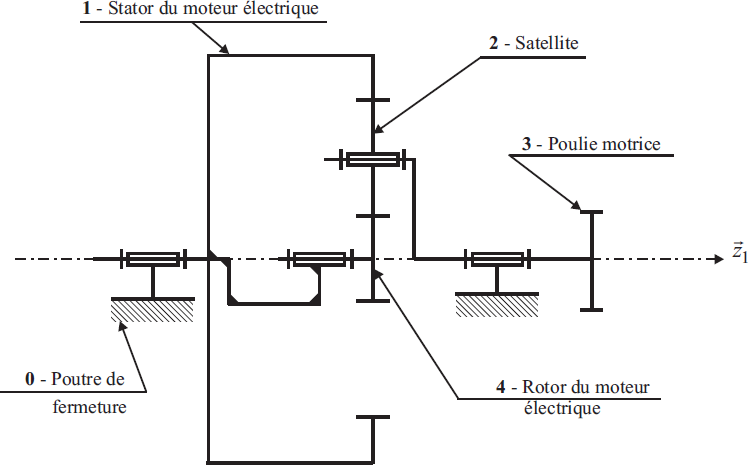
\includegraphics[width=\linewidth]{983_01}%
\end{center}


\subsubsection*{Étape de louvoiement}
Pendant la phase de louvoiement, pour une vitesse du vantail par rapport à la
poutre de fermeture de $||\vect{V}_{\text{vantail}/\text{poutre}} || = \SI{0,5}{m.s^{-1}}$, la vitesse de rotation du
moteur passe par un maximum. À cet instant, la vitesse de translation de la
poutre de fermeture par rapport à la voiture suivant $\vect{y}$ est de $\SI{0,15}{m.s^{-1}}$; ce qui
donne une vitesse de rotation du stator $||\Omega_{1/0}\vect{z_1}||=\SI{7,3}{rad.s^{-1}}$.

\subparagraph{}
\textit{Déterminer l’expression de la vitesse du moteur en fonction $\Omega_m$ en fonction de $\Omega_{1/0}$, $\Omega_{3/0}$, $Z_1$ et $Z_4$.}
\ifprof
\begin{corrige}
\end{corrige}
\else
\fi

\subparagraph{}
\textit{Effectuer l’application numérique et vérifier la conformité au cahier des charges du moteur : $\omega_{\text{max}}=\SI{1000}{tr.min^{-1}}$. }
\ifprof
\begin{corrige}
\end{corrige}
\else
\fi

Application numérique : $\Phi_p = \SI{80}{mm}$, $Z_1 = \SI{60}{dents}$, $Z_4 = \SI{10}{dents}$.

\subsubsection*{Étape de verrouillage}

\subparagraph{}
\textit{Déterminer l’expression de la vitesse du moteur $\Omega_m$ en fonction de $\Omega_{1/0}$, $Z_1$, $Z_4$.}
\ifprof
\begin{corrige}
\end{corrige}
\else
\fi

\subsubsection*{Étape de coulissement}

Pendant la phase de coulissement, la vitesse des vantaux par rapport à la poutre
de fermeture est égale à $\vect{V}_{\text{vantail}/\text{poutre}}=v\vect{x}$.



\subparagraph{}
\textit{Donner l’expression de la vitesse du moteur $\Omega_m$ en fonction de $v$, $\Phi_p$, $Z_1$, $Z_4$.}
\ifprof
\begin{corrige}
\end{corrige}
\else
\fi

\subparagraph{}
\textit{En supposant que les phases de louvoiement et de verrouillage ont une durée
totale de \SI{1,5}{s}, vérifier que la vitesse maximale du moteur, permet d’assurer le temps de fermeture
exigé par le cahier des charges.}
\ifprof
\begin{corrige}
\end{corrige}
\else
\fi

On rappelle que pendant l’étape de coulissement l’écartement des vantaux
passe de \SI{1300}{mm} à \SI{200}{mm}.

%
%\subparagraph{}
%\textit{}
%\ifprof
%\begin{corrige}
%\end{corrige}
%\else
%\fi
%


\begin{enumerate}
\item $\Omega_m = \Omega_{4/1}=\left(\Omega_{3/0}-\Omega_{1/0} \right) \dfrac{Z_1 + Z_4 }{Z_4}$.
\item $\Omega_{m}=\Omega_{4/1}=\SI{348}{tr.min^{-1}}$.
\item $\Omega_m = \Omega_{4/1}=\left(-\Omega_{1/0} \right) \dfrac{Z_1 + Z_4 }{Z_4}$.
\item $\Omega_m = \Omega_{4/1}=\dfrac{2v \left(Z_4 + Z_1\right)}{\Phi_P Z_4}$.
\item $\Omega_m = \SI{613}{tr.min^{-1}}$.
\end{enumerate}
